\documentclass[conference]{IEEEtran}
\IEEEoverridecommandlockouts
% The preceding line is only needed to identify funding in the first footnote. If that is unneeded, please comment it out.
\usepackage{cite}
\usepackage{amsmath,amssymb,amsfonts}
\usepackage{algorithmic}
\usepackage{graphicx}
\usepackage{textcomp}
\usepackage{xcolor}
\def\BibTeX{{\rm B\kern-.05em{\sc i\kern-.025em b}\kern-.08em
    T\kern-.1667em\lower.7ex\hbox{E}\kern-.125emX}}
\begin{document}

\title{Enter Title here\\
{\footnotesize Université Paris-Saclay Machine Vision Project}
\thanks{Identify applicable funding agency here. If none, delete this.}
}

\author{\IEEEauthorblockN{Charbel Abi Hana}
\IEEEauthorblockA{\textit{Department of Electrical Engineering} \\
\textit{Université Paris-Saclay}\\
Paris, France \\
charbel-a-h@outlook.com}
}

\maketitle

\begin{abstract}

\end{abstract}

\begin{IEEEkeywords}

\end{IEEEkeywords}

\section{Introduction}


\section{Related Work}


\section{Methods}

\subsection{Conditional Generative adversarial network(GANs)}%Change it to urs


\begin{equation}
\min_{G}\max_{D}\mathcal V_{\text{GAN}}\left(D, G \right) = \end{equation}
\begin{align*}
 \mathbb E_{x \sim p_{\text{data}\left( x\right) }}\left[ \log \left\{ D\left( x \right) \right\} \right] + \mathbb E_{z\sim p_{z}\left( z\right)}\left[ \log\left\{ 1 - D\left( G\left( z\right) \right) \right\}\right].   
\end{align*}

where \begin{math}G : R^{100} \longrightarrow R^{16,384}\end{math}
\begin{equation}
L_D = - \sum_{x \in \chi, z \in \zeta} \log(D(x)) + \log(1 - D(G(z))) \tag{6}
\end{equation}
\begin{equation}
L_G = - \sum_{z \in \zeta} \log(D(G(z)) \tag{7}
\end{equation}

\subsection{Model Architecture}

\subsubsection{Generator}

\begin{equation}
h^{[i]} = LeakyRELU(W^{[i-1]}h^{[i-1]}+b{[i-1]})\label{Gen LeakyRELU}
\end{equation}
\begin{math}\alpha \end{math}, with h[i] \begin{math}\epsilon R^{16\alpha2^i}\end{math} and we output the vector o \begin{math}\epsilon R^{16,384}\end{math} via
\begin{equation}
o =tanh(W^{[L]}h^{[L]}+b{[L]})
\end{equation}
Where L is the final layer.

\subsubsection{Discriminator}
\begin{math}h[0]\end{math} denote the input
image, \begin{math}W [j]\end{math} and \begin{math}b[j]\end{math} denoting the weight matrix and the bias vector in the L output layer, we have:
\begin{equation}
o = sigmoid(W^{[L]}h^{[L]}+b{[L]})
\end{equation}


\subsubsection{Classifier}

\section{Experiments}
\subsection{Dataset}

\begin{figure}[htbp]
\centerline{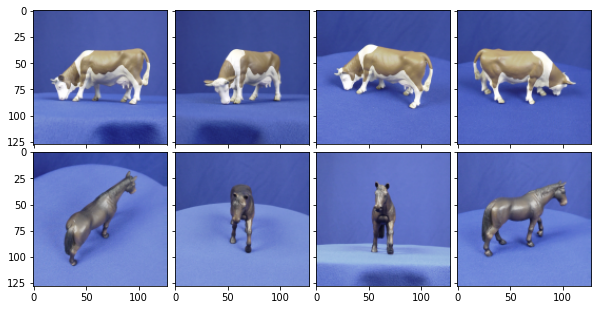
\includegraphics[width=75mm]{1.png}}
\caption{Random Cows and Horses Images from Original Dataset}
\label{fig}
\end{figure}

\subsection{Evaluation Metrics}\label{AA}


\subsection{Experimentation Details}


\subsection{GAN Experimentation Results}

\begin{figure}[htbp]
\centerline{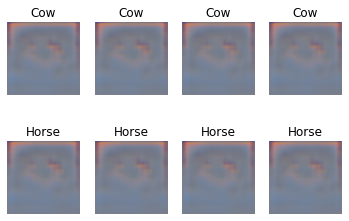
\includegraphics[width=75mm]{2.png}}
\caption{Generated Output after 100 Steps}
\label{fig}
\end{figure}

\begin{figure}[htbp]
\centerline{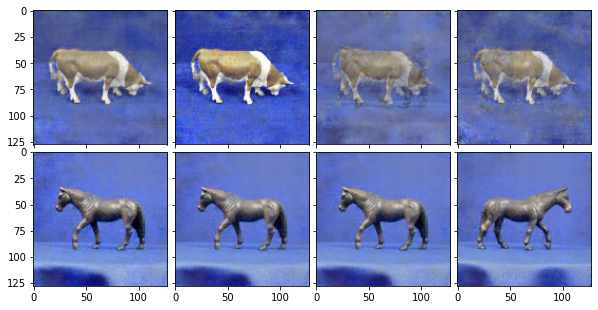
\includegraphics[width=75mm]{3.png}}
\caption{Generated Output after 35000 Steps}
\label{fig}
\end{figure}


\begin{figure}[htbp]
\centerline{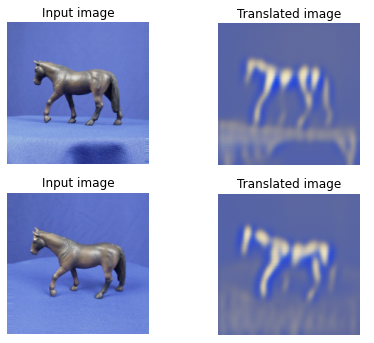
\includegraphics[width=60mm]{5.png}}
\caption{Generated Translated Output after 1 Epoch}
\label{fig}
\end{figure}

\subsection{CycleGAN Experimentation Results}

\begin{itemize}
    \item Pass real images through the generators and get the generated images
    \item Pass the generated images back to the generators to check if we can predict the original image from the generated image.
    \item Do an identity mapping of the real images using the generators.
    \item Pass the generated images in 1) to the corresponding discriminators.
    \item Calculate the generators total loss (adverserial + cycle + identity)
    \item Calculate the discriminators loss
    \item Update the weights of the generators
    \item Update the weights of the discriminators
    \item Return the losses in a dictionary.
\end{itemize}


\begin{figure}[htbp]
\centerline{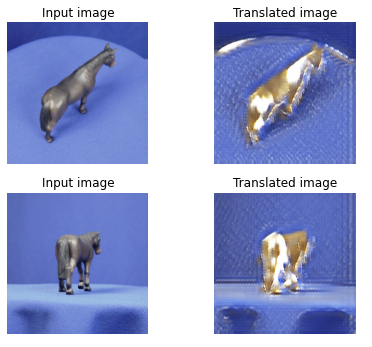
\includegraphics[width=60mm]{4.png}}
\caption{Generated Output after 50 Epochs}
\label{fig}
\end{figure}

\subsection{Classifier Experimentation Results}

\begin{figure}[htbp]
\centerline{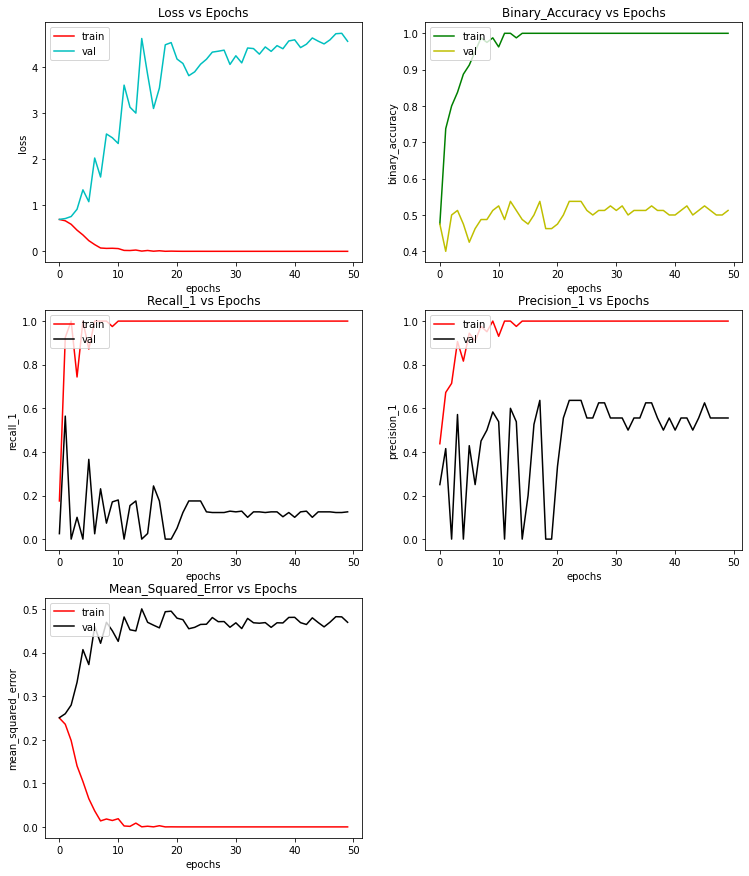
\includegraphics[width=80mm]{plot_orig.png}}
\caption{Classification metrics for classifier trained on \textbf{original dataset}}
\label{fig}
\end{figure}

\begin{figure}[htbp]
\centerline{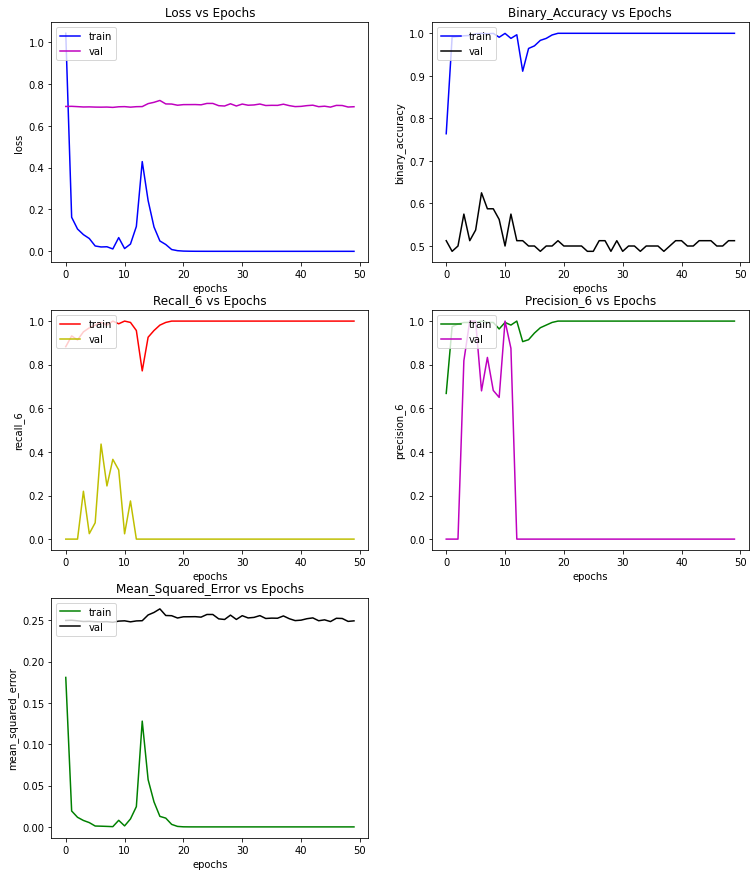
\includegraphics[width=80mm]{plot_250.png}}
\caption{Classification metrics for classifier trained on \textbf{original+250 GAN-based}}
\label{fig}
\end{figure}


\begin{figure}[htbp]
\centerline{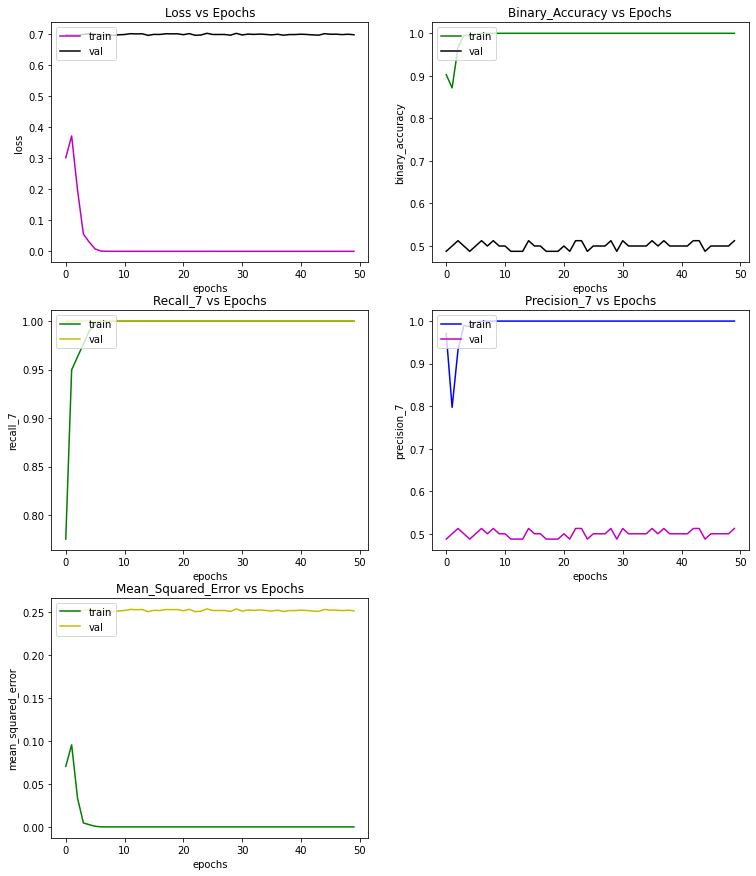
\includegraphics[width=80mm]{plot_500.png}}
\caption{Classification metrics for classifier trained on \textbf{original+250 GAN-based}}
\label{fig}
\end{figure}

\begin{figure}[htbp]
\centerline{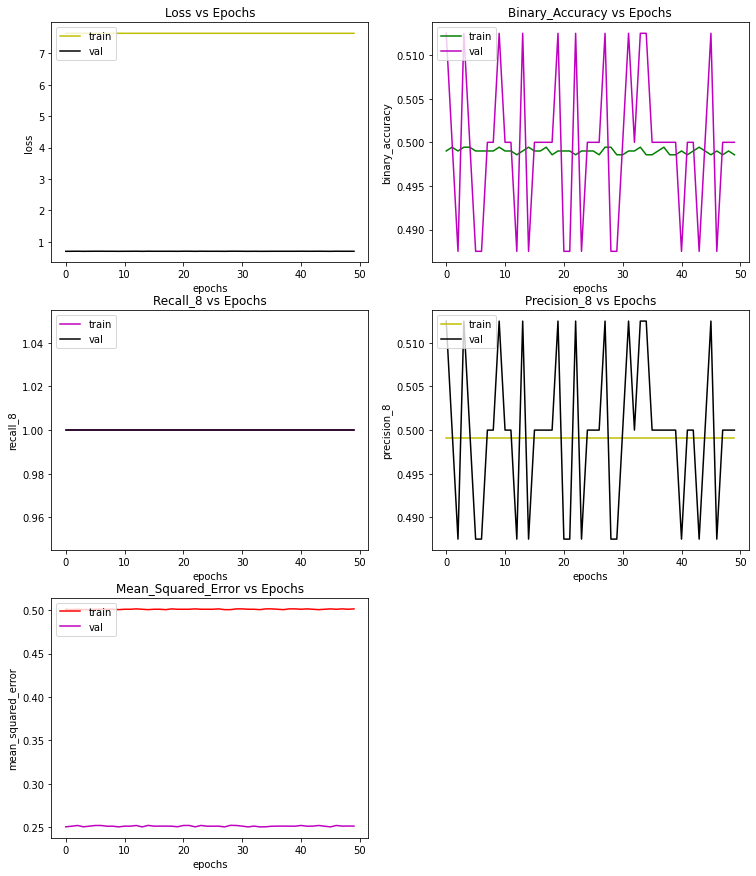
\includegraphics[width=80mm]{plot_1000.png}}
\caption{Classification metrics for classifier trained on \textbf{original+250 GAN-based}}
\label{fig}
\end{figure}

\begin{table}[h!]
\centering
\begin{tabular}{| *{9}{c|} }
    \hline
\textbf{Metric}    & \multicolumn{2}{c|}{Orig}
            & \multicolumn{2}{c|}{Orig-250-GAN}
                    & \multicolumn{2}{c|}{Orig-500-GAN}
                            & \multicolumn{2}{c|}{Orig-1000-GAN}                \\
    \hline
-   &   \textbf{train}  &   \textbf{val}  &   \textbf{train}  &   \textbf{val}  &   \textbf{train}  &   \textbf{val}  &   \textbf{train}  &   \textbf{val}  \\
    \hline
BCE-Loss   &   0.01  &   5  &   0.01  &   0.7  &  0.01   &  0.7   &   8  &  0.7   \\
    \hline
Accuracy   &    1.0   &     0.5  &   1.0    &     0.6  &   1.0    &    0.5   &   0.5    &   0.5    \\
    \hline
Precision   &   1.0    &   0.1    &   1.0    &    0.5   &   1.0    &    0.5   &   0.5    &    0.5   \\
    \hline
Recall   &    1.0   &    0.5   &    1.0   &   0.4   &    1.0   &    1.0   &    1.0   &  1.0     \\
    \hline

\end{tabular}
\caption{Compiled table of Classification Metrics}
\end{table}

\section{Conclusion}



\bibliographystyle{plain} % We choose the "plain" reference style
\bibliography{citations} % Entries are in the refs.bib file
\end{document}
